\documentclass[centeredchapter]{thesis-ekf}
\usepackage[T1]{fontenc}
\usepackage[utf8]{inputenc}
\PassOptionsToPackage{defaults=hu-min}{magyar.ldf}
\usepackage[magyar]{babel}
\usepackage{graphicx,amsmath,amssymb,amsthm}
\graphicspath{{./images/}}
\footnotestyle{rule=fourth}

\newtheorem{tetel}{Tétel}[chapter]
\newtheorem{lemma}[tetel]{Lemma}
\theoremstyle{definition}
\newtheorem{definicio}[tetel]{Definíció}
\newtheorem{feladat}[tetel]{Feladat}
\theoremstyle{remark}
\newtheorem{megjegyzes}[tetel]{Megjegyzés}
\newtheorem*{megoldas}{Megoldás}
\usepackage{listingsutf8,xcolor,caption}
\lstset{
	inputencoding=utf8/latin2,
	language=Java,
	basicstyle=\footnotesize,
	numbers=left,
	breaklines,
	postbreak=\hbox{},
	xleftmargin=2cm,
	xrightmargin=2cm,
	backgroundcolor=\color{white},
	frame=tlbr,
	framesep=1pt,
	keywordstyle=\bfseries\color{blue},
	commentstyle=\itshape\color{green}
}
\renewcommand{\lstlistingname}{kód}

\usepackage{xcolor}
\usepackage{listings}

\definecolor{dkgreen}{rgb}{0,.6,0}
\definecolor{dkblue}{rgb}{0,0,.6}
\definecolor{dkyellow}{cmyk}{0,0,.8,.3}
\definecolor{gray}{rgb}{0.5,0.5,0.5}
\definecolor{mauve}{rgb}{0.58,0,0.82}

\lstdefinestyle{Java}
{	
	language=Java,
	aboveskip=3mm,
	belowskip=3mm,
	showstringspaces=true,
	columns=flexible,
	basicstyle={\small\ttfamily},
	numbers=left,
	numberstyle=\tiny\color{gray},
	keywordstyle=\color{blue},
	commentstyle=\color{dkgreen},
	stringstyle=\color{mauve},
	breaklines=true,
	breakatwhitespace=true,
	tabsize=3
}


\logo{
\includegraphics[width=9cm]{ekf-logo3}}
\institute{Matematikai és Informatikai Intézet}
\title{Szoftverfejlesztés Java Enterprise platformon}
\authorcaption{Készítette:}
\author{Kosárkó Ákos \\ Programtervező informatikus Bsc szak}
\supervisorcaption{Témavezető:}
\supervisor{Tajti Tibor\\ tanársegéd}
\city{Eger}
\date{2016}

\begin{document}
\maketitle
\tableofcontents


\chapter*{Bevezetés}

2015 elején foglalkoztatni kezdett, hogy munkába álljak és pénzt keressek. Ezen célért az interneten böngészve rátaláltam egy iskolaszövetkezet hirdetésére, amely biztos munkát ígért az általuk kínált képzés elvégzése után. A képzés tárgyaként a JAVA EE volt megjelölve, amiről első körben nem tudtam, hogy micsoda, annyit sejtettem, hogy a Java programozási nyelvhez kapcsolódhat. Második nekifutásra utánaolvastam az interneten, az jött le, hogy ez a Java programozási nyelv rengeteg külső osztálykönyvtárral kibővített "változata". Ma már tudom, hogy ez ennél jóval több. Visszatérve az iskolaszövetkezet hirdetésére, kapva az alkalmon, jelentkeztem a hirdetésükre, és a felvételi interjú után alkalmasnak találtak arra, hogy részt vegyek a képzésükön. 

Így kerültem kapcsolatba a Java Enterprise Edition technológiával, amely, mint később világossá vált számomra, az iparban széles körben elterjedt és számos helyen használt eszköz. A szakdolgozat elkészítésével és az ehhez írt alkalmazás elkészítésével célom a technológia általam már ismert részének bemutatása, a technológia által nyújtott és számomra új megoldások megtalálása, és a gyakorlás. Mindezeket egy fiktív telekommunikációs cég számára készített alkalmazás, amellyel online ügyintézést tesznek lehetővé a régi és új ügyfeleik számára.

\chapter{Az alkalmazás bemutatása}

\section{Az alkalmazás működtetésének célja}

Az alkalmazás működtetésének célja lehetővé tenni a szolgáltató ügyfelei számára, hogy online intézhessék az ügyeiket. Ezen ügyintézésbe a cég szolgáltatásaira való előfizetés, számlabefizetés és hibabejelentés tartozik, emellett az alkalmazást a szolgáltató ügyintézői szintén használhatják, akik az ügyintézői jogosultságuk miatt más tartalomhoz férnek hozzá, mint az ügyfelek. Ők látják az összes bejelentett hibajegyet, amikhez a hiba elhárításának megoldását fűzik hozzá a hibabejelentés lezárásaként. 

\section{Képernyők}

Az alkalmazással végezhető műveletek természetesen láthatóak kell legyenek a használóik számára, erre a képernyők szolgálnak. Az alkalmazás webes böngészőkön keresztül érhető el a felhasználók számára, a képernyők is abban fognak megjelenni nekik. Az alábbiakban a felhasználók számára megjelenő képernyők leírását adom meg.
A képernyők két csoportba bonthatók:
 
 \begin{itemize}
 	\item Az egyik csoportba azok a képernyők tartoznak, amelyek bárki számára(azaz a nem bejelentkezett felhasználók számára is) megjelennek. Az ezeken a képernyőkön elérhető információk és műveletek nincsenek egyénekhez kötve, egyedi információkat nem tartalmaznak. Ezzel együtt vannak olyan bárki számára elérhető oldalak, amelyek bejelentkezés után bővebb tartalommal rendelkeznek.
 	\item Ennek ellenkezője áll fenn a bejelentkezett felhasználók számára elérhető oldalak esetén. Ezeken az oldalakon olyan információk és műveletek is elérhetőek, amelyek egyéniek, azaz bejelentkezett felhasználónként különböznek. Ilyen például a számlák képernyő, ahol nyilvánvalóan a felhasználó saját számlai kerülnek megjelenítésre. Ennek adatvédelmi okai vannak: egy előfizető számláit csakis ő maga láthassa, az alkalmazás többi felhasználója ne.
 	A bejelentkezett felhasználók típusoktól függően (ügyfél illetve ügyintéző) más felületeket érnek el: egy ügyfél hibabejelentő oldalt ér el, míg az ügyintéző a bejelentett hibákat listáztathatja ki, és kezelheti.
 \end{itemize}
  

\subsection{Főoldal}\hypertarget{leiras-fooldal}{}

Az alkalmazás kezdőoldala a főoldal, amely a bárki számára megjelenő oldalakhoz közé tartozik. Ez az oldal egy rövid üdvözlő szöveget jelenít meg, a bárki számára elérhető menüpontok gombjaival együtt.

\subsection{Regisztrációs oldal}\hypertarget{leiras-regisztracios}{}

Az oldalon történő ügyintézéshez egy saját felhasználói fiókra szükséges. Ezt a fiókot a \hyperlink{leiras-regisztracios}{"Regisztrációs oldal"}-on hozhatja létre a leendő ügyfél, amelyre a képernyő jobb felső sarkában lévő login-box "Regisztráció" linkre kattintással jut el. A fiók létrehozásához személyes adatainak megadására van szükség, amely a form mezőinek kitöltésével végzendő el. A megadott adatok a regisztráció véglegesítése előtt egy validáción kell hogy keresztül menjenek. A validáció célja jelen esetben az, hogy elkerüljük olyan értékek megadását, amik nem lehetnek valósak, például egy számjegy a névben. 

\subsection{Bemutatkozás}\hypertarget{leiras-bemutatkozo}{}

A \hyperlink{leiras-bemutatkozo}{"Bemutatkozó oldal"}-on a szolgáltató hosszabb bemutatkozása olvasható, amely bővebb információkat ad a működéséről, felépítéséről és az általa nyújtott szolgáltatásokról.

\subsection{Szolgáltatások}\hypertarget{leiras-szolgaltatasok}{}

A \hyperlink{leiras-szolgaltatasok}{"Szolgáltatások"} felület egy fontos felület a képernyők között. Ezen a felületen találja meg az oldal látogatója a cég által nyújtott szolgáltatások listáját és azok jellemzőit, úgy mint az ár, internetszolgáltatás esetén a sebesség, stb. Mivel a cég többféle szolgáltatást is nyújt(telefon, internet, kábeltv) ezért az oldal áttekinthetősége és a szolgáltatások megjelenítésének struktúrája kiemelkedő fontosságú. Éppen ezért a szolgáltatások listája szolgáltatástípusonként megjelenítve áll rendelkezésre az ügyfelek számára.
A bejelentkezett felhasználók itt adhatják hozzá a bevásárlókosarukhoz a szolgáltatásokat, amelyekre elő kívánnak fizetni. A bevásárlókosárba tett szolgáltatások megrendelését a "Megrendel" gomb megnyomásával eszközölheti az ügyfél, ami után a szolgáltatási végpont adatait kell hogy megadja. A megrendelt szolgáltatások az itt megadott címre kerülnek bekötésre.

\subsection{Kapcsolat}\hypertarget{leiras-kapcsolat}{}

A \hyperlink{leiras-kapcsolat}{"Kapcsolat"} oldalon a cég elérhetőségei olvashatóak, úgy mint a székhely, ügyfélszolgálati telefonszám és levelezési cím.

\subsection{Számlák}\hypertarget{leiras-szamla}{}

Ez az oldal az előfizetések megléte miatt kiállított számlákat listázza ki. Az ügyfél minden egyes befizetetlen számláját kilistázásra kerül ezen a felületen, számlanévvel, összeggel és befizetési határidővel együtt. A számla befizetésére bankkártyás fizetéssel van mód, amelyhez a bankkártyán szereplő adatokat a számlához tartozó befizetés gomb megnyomásával betöltődő oldalon kell megadni. Ezen az oldalon - természetesen egy kitalált, nem létező - pénzügyi szolgáltató felé történő kérés fut le, amely a bankkártyás fizetést szimulálja. Ez a fizetési kísérlet kétféle eredménnyel záródhat:
 Az ügyfél bankszámláján van elegendő pénz a számla kiegyenlítésére, és ez esetben a számla befizetett státuszba kerül.
 A másik eset az, amikor az ügyfél bankszámláján nem áll rendelkezésre elegendő pénz a számla befizetésére, így az befizetésre váró számlaként marad a számlák között.
 Mivel nincs valós pénzügyi szolgáltató a befizetések mögött, ezért a befizetés sikerességét vagy sikertelenségét egy véletlen szám generálással határozom meg, amelynek értéke dönti el, hogy sikeres vagy sikertelen legyen a befizetés. Mindkét esetben újra a \hyperlink{leiras-szamla}{"Számlabefizetés"} oldal töltődik be újra.

\subsection{Hibabejelentés}\hypertarget{leiras-bejelentes}{}

Az aktív szolgáltatással rendelkező felhasználóknak lehetőségük nyílik a szolgáltatással kapcsolatos hibák bejelentésére. Ezt a \hyperlink{leiras-bejelentes}{"Hibabejelentés"} oldalon tehetik meg.
Az észlelt hiba részleteit egy form kitöltésével adhatják meg, amely form beküldésével az rögzítésre kerül, és az ügyintézők számára láthatóvá válik.

\subsection{Bejelentett hibák}\hypertarget{leiras-bejelentetthibak}{}

Ez egy az ügyintézők számára elérhető felület, amin a még ki nem javított hibákról szóló bejelentések érhetőek el. Amennyiben egy hiba kijavításra került, azt az ügyintézők a megoldást eredményező munkálatok rögzítésével nyugtázhatják.

\section{A szoftver elkészítésére használt technológiák, és az azt támgató eszközök}

Egy alkalmazás elkészítése összetett folyamat. Ennek során nem elég a specifikációt ismerni, és az alkalmazott programozási nyelv használatában járatosnak lenni, ezek mellet számos olyan eszközt érdemes igénybe venni, amely gyorsítja, hatékonyabbá, vagy éppen "biztonságosabbá" teszi az alkalmazás fejlesztését azáltal, hogy a szoftverkészítés folyamat egyes állomásain a forráskód állapotát eltárolja.

\subsection{Java Enterpreise Edition}

A szakdolgozatom témája a Java EE technológia bemutatása, így ez az a technológia, amiről részletesen írni fogok. Bevezetésül pár dolgot írok itt a technológiáról.

A Java Enterprise Edition API-k egy halmaza, amely API-k lehetővé teszik nagy skálázhatósággal rendelkező üzleti alkalmazások elkészítését. 13 API van, amelyek a technológia részeiül szolgálnak.
Egy alkalmazás elkészítéséhez nem szükséges minden API-t felhasználni. Például abban az esetben, amikor az alkalmazásunkban nincs szükség a kliensek közötti üzenetküldésre, abban az esetben a JMS -Java Message Service - használata nélkülözhető.

Természetesen vannak olyan API-k amelyek használata szinte nélkülözhetetlen a JEE technológia felhasználásával készített alkalmazások során. Ezen API-k az EJB és a JPA API-k, amik az üzleti logika és az adatbázisműveletek implementálására alkalmasak.

Az általam készített alkalmazás egy olyan alkalmazás, amelyik az API-k egy részét fogja használni.

\subsection{WildFly Application Server}

Az elkészült alkalmazások futtatásához egy olyan környezet szükséges, amely ismeri és kezeli az alkalmazás által használt API-kat. Ezeket a környezeteket az alkalmazásszerverek. 
Feladatuk az alkalmazás számára biztosítani az általa használt API-kat, és erőforrás kezelést, erőforrás (ki)osztást végezni. Ilyen erőforrás (ki)osztás alatt értem például az alkalmazásszerver azon műveleteit, amelynek során az erőforrás konténerekbe annyi EJB példányt tárol, amennyi a kliensoldalról érkező kéréseket (optimálisan) képes kiszolgálni.

Én a WildFly alkalmazásszervert fogom használni, amely a JBoss alkalmazásszerver community verziójának új neve a 8.0-s verzió óta. Ez az alkalmazásszerver alkalmas a Java EE technológiával készült alkalmazások futtatására, mert implementálja annak összes standardját.  

\subsection{Oracle Database 11g Express Edition}

Az alkalmazás a felhasználókról, szolgáltatásokról, stb adatokat tárol. Erre az Oracle ingyenesen használható adatbázisát, az Oracle Database 11g Express Edition-t használja.
\subsection{IntelliJ IDEA}

A fejlesztői környezetnek az IntelliJ IDEA nevű eszközét választottam. Ezen választásom oka az, hogy tapasztalt programozóktól azt hallottam, hogy a forgalomban lévő fejlesztői környezetek közül ez a tapasztalataik alapján az egyik legjobb. Ezen választás hozomány, hogy egy újabb fejlesztői környezetet ismerek meg, a főiskolai tanulmányaim során használt Microsoft Visual Studio és NetBeans mellett.

\subsection{Vaadin Framework}

Az alkalmazás frontend részét Vaadin Framework használatával fogom elkészíteni. Ennek oka az, hogy Java-alapú frontend készítést tesz lehetővé. Ez azt jelenti, hogy a böngészőben megjelenő oldalakat nem HTML használatával kell összeállítani, hanem a framework által nyújtott Java objektumokkal, és az így összeállított oldalak HTML5-ként generálódnak ki, amelyet a böngészők képesek megjeleníteni.

\subsection{Maven}

A szoftverfejlesztési iparban jelenleg sok programozó és sok cég van jelen. Előfordul, hogy az egyikük elkészít egy funkcióhalmazt implementáló kódot, és azt mások által felhasználhatóvá teszi.
Az is előfordulhat, hogy egy specifikációt, elvbeli működést (pl JPA) több cég is implementál, méghozzá másként, majd kiadja azt másoknak felhasználásra. Ezen esetekben ezeken az implementációkat osztálykönyvtárak formájában érjük el egy központi repositoryban. Amennyiben használni szeretnénk ezen osztálykönyvtárakat, elérhetővé kell tennünk ezeket a projektünk számára, mivel az függ azoktól. Ez esetben jön jól a Maven, amellyel a projektünk függőségei könnyen letölthetők az internetről és hozzáadhatók a projektünkhöz. Ehhez mindössze egy megfelelő módon összeállított, projektfüggőségeket leíró fájlra van szükségünk.(pl pom.xml) Ez a fájl tartalmazza a projektben használt függőségek elérési helyét és azonosítóját, így azok egy áttekinthető, struktúrált és kényelmes módon integrálhatóak a projektünkbe.

\subsection{Git}

A program elkészítése során nagy segítséget nyújt egy verziókezelő rendszer használata, amely lehetővé teszi a fejlesztés során az alkalmazás aktuális állapotának mentését. Ennek több előnye is van. Egyik előnye az, hogy a fejlesztés egy pontjából több irányba is elágaztathatjuk a a fejlesztés további menetét. Ez amiatt hasznos, mert ha két megrendelő hasonló alkalmazást kér, akkor az alkalmazások funkciói közötti átfedéseket egy fejlesztési vonalon kezelhetjük és implementálhatjuk, a különbségeket pedig egy-egy külön ágon "adhatjuk" hozzá az átfedéseket tartalmazó részhez. Másik előnye a verziókezelésnek, hogy amennyiben azt találjuk, hogy az alkalmazás jelenlegi állapota nem a kívánt állapottal egyenlő, akkor könnyen átállhatunk egy olyan mentett állapotra, amelyik egy kívánt állapot. Harmadik előnye, hogy amennyiben osztott verziókezelő rendszert használunk, úgy a forráskódból több példány is van, így az esetben, ha az egyik példány elveszne, úgy tényleges veszteség nem ér minket, mivel a projekt kódja máshol is tárolva van.

Én egy a github-on létrehozott repositoryt és a Git nevű verziókezelő rendszert használom az alkalmazás elkészítése során.


\chapter{A Java Enterprise Edition}

\section{Mi a Java EE?}

A jelen korban gyakori eset, hogy olyan szoftvereket kell készítenünk, amelyek a felhasználóik számára rengeteg funkciót biztosítanak, és emellett megbízhatónak és biztonságosnak is kell lenniük. Ahhoz , hogy ezeket az igényeket kielégítsük, és az alkalmazásunk viszonylag rövid idő alatt elkészüljön, az szükséges, hogy a szoftver elkészítéséhez szükséges építőkockát közül ne az összeset mi írjuk meg, vagyis felhasználhassunk olyan eszközöket, építőkockákat, amiket mások már elkészítettek, ezáltal mi már nagyrészt csak ezek összeillesztésére kell, hogy időt és energiát fordítsunk, ami összetett alkalmazások esetében még így is jelentős mennyiségű. 
Például, teljesen felesleges minden egyes alkalmazásunkban elkészíteni egy típust, ami primitív típusú elemeket tartalmaz, hiszen ezt már másvalaki(k) elkészítették, és a műveleteit optimalizálták. Ezek a listák, mint egy alkalmazás építőkockái. Ez, és sok más építőkocka API-ként a Java Standard Edition-jében található meg összegyűjtve.
Ennek mintájára, robosztus méretű alkalmazások elkészítéséhez nagy méretű építőkockákat is elkészítettek, amelyek összetett műveletek elvégzésére alkalmasak. Ezekkel az építőkockákkal néhány 10 sor általunk írt programkóddal elvégezhető egy entitás adatbázisba történő perzisztálása, alkalmazások közötti üzenetküldés, e-mail küldés, és egyéb összetett művelet, amelyeket ha mi kellene, hogy megírjunk, nagy mértékben megnövekedne a fejlesztéshez szükséges időtartam.
Ezeket a nagy építőkockákat gyűjtötték össze, mint API-k, amiből létrejött a Java EE.
Ez az enterprise edition a standard edition teljes egészét felhasználhatja, illetve ha egy Java EE alkalmazást készítünk, mi is használhatjuk benne a Java SE tartalmát.

\section{Arhitektúra}

A Java EE különböző konténerekben implementált specifikációk halmaza. A konténerek Java EE futtatói környezetek, amelyek különböző szolgáltatásokat bitosítanak az általuk kiszolgált komponenseknek. Ilyen szolgáltatások például az életciklus menedzselés, a függőség befecskendezés, és így tovább. Ezek a komponensek jól definiált szerződéseket használnak a Java EE infrasruktúrabeli kommunikációhoz, és más komponensekkel történő kommunikációhoz egyíránt. Deploy-olás (az alkalmazásszerverre történő kihelyezés) előtt úgynevezett package-ekbe csomagolandóak, amik típusát és kiterjesztését a célkonténer típusa határoz meg.

\begin{figure}[!h]
	\centering
	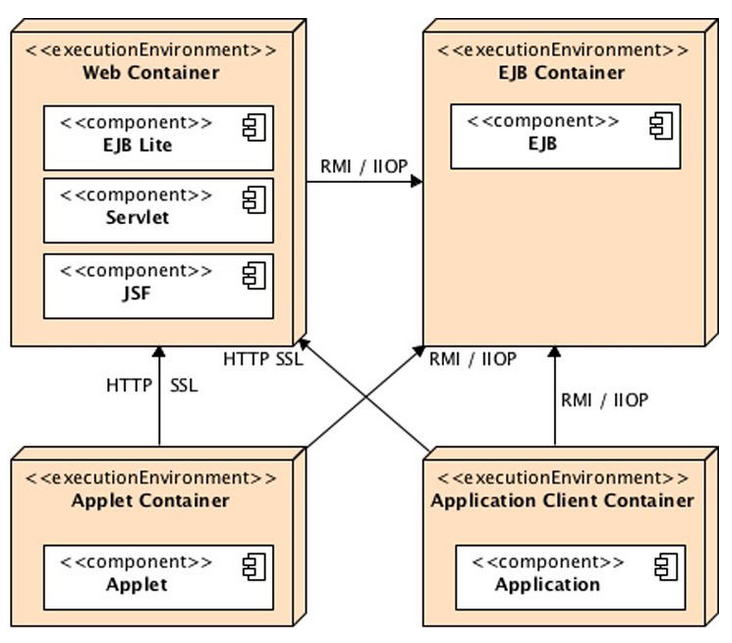
\includegraphics[width=14cm]{kontenerek.png}
\end{figure}

Az alábbi ábrán a platform négy konténere látható, a köztük lévő kapcsolódási protokollok megjelölésével.

\section{Komponensek}

\subsection{Komponensek bemutatása}
A platform négy komponenstípust tartalmaz:
\begin{itemize}
	\item Applet: grafikus felhasználói felülettel(Graphic User Interface - GUI) rendelkező alkalmazások, amelyek webes böngészőkben futnak.
	
	\item Application: olyan programok, amelyek kliens gépeken futnak. Ezek tipikusan GUI-k, amelyeknek a Java EE középső rétegének összes eszközéhez elérése van.
	
	\item Web Applicaton: servletekből, JSP-kből, JSF-ekből, stb állnak, a web konténerben futnak, és a kliensekből érkező kéréseket szolgáljak ki.
	
	\item Enterprise Application: az EJB konténerben futtatjuk. Ezek az alkalmazások EJB-kből (Enterprise Java Beans), Java Message Service-ből, Java Transaction API-ból, asszinkron hívásokból, RMI/IIOP-ből állnak. Az EJB-k konténer-menedzselt komponensek, amelyek az üzleti logikát írják le és implementálják. Lokálisan, vagy RMI-n keresztül távolról érhetőek el. 
	
\end{itemize} 

\subsection{Komponensek csomagolása}

Ahhoz, hogy egy komponenst kihelyezhessünk a szerverre, először be kell, hogy csomagoljuk egy standard formátumba. A Java SE a Java Archive (jar) fájlokat használja erre, amelyek több fájl (Java osztályok, deployment descriptorok, erőforrások, külső könyvtárak) egyetlen fájlba csomagolásai. Ez a csomagolás ZIP formátum alapú.
Minden egyes modul számára meghatározott, hogy milyen típus csomagolt fájlba kell csomagolni:
\begin{itemize}
	\item Az application client modul java osztályokat és más erőforrás fájlokat tartalmaz, amiket egy .jar fájlba kell csomagolni.
	
	\item Az EJB modulok egy vagy több bean-t tartalmaznak, és esetükben szintén a .jar kiterjesztés a megkövetelt.
	
	\item A web application module számos elemet tartalmazhat: servleteket, JSP-ket, JSF-eket, Java-Scriptet, HTML fájlokat, CSS-t, stb. Mindezek egyetlen Web-Archive fájlba kerülnek, ami egy .war kiterjesztésű állomány.
	
	\item A negyedik modultípus az enterprise modul, ami bármennyi (akár 0-t is) web modul-t(.war), bármennyi EJB modult(.jar) tartalmazhat, és mindezeket egy Enterprise Archive .ear kiterjesztésű fájlban fogja össze.
	
\end{itemize} 

\section{Konténerek}

\subsection{Konténerek leírása}

A Java EE infrastruktúra logikai egységekbe került felosztásra, amiket konténereknek nevezünk. Minden egyes konténernek speciális szerepe van, má-más szolgáltatásokat tesznek elérhető a komponensek számára. A konténerek elrejtik a technikai komplexitást.
Attól függően, hogy milyen típusú alkalmazást akarunk fejleszteni, más és más konténer(eke)t kell használnunk. Például, ha egy webes alkalmazást fejlesztünk, akkor elegendő egy JSF réteget és egy EJB Lite réteget fejleszteni, amik a web konténerbe deployolva működőképesek.
Négy különböző konténer létezik:
\begin{itemize}
	\item Az Applet konténer applet komponensek futtatására alkalmas. Homokozó biztonsági modell-t használ, így a kód egy homokozó környezetben fut, és a "homokozóm kívüli játék" nem megengedett.
	Ez azt jelenti, hogy a konténer megelőzi azt, hogy az applet a lokális gépen lévő erőforrásokhoz -képekhez, fájlokhoz- hozzáférjen.
	\item Az Application Client Container Java osztályokat, könyvtárakat és egyéb fájlokat tratalmaz, amik ahhoz szükségesek, hogy a Java SE alkalmazás egy EJB konténerbeli vagy egy Web konténerbeli komponenssel képes legyen kommunikálni.
	\item A Web konténer web komponensek futtatásának és menedzselésének alapjául szolgáló szolgáltatásokat biztosítja. Például ez a konténer felelős az EJB-k példányosításáért, inicializálásáért és a servlet hívásokért. HTTP és HTTPS protokollon keresztül érhető el. Ez az a konténer, amit a web oldalak generálására használunk, amik ezután eljutnak a böngészőbe.
	\item Az EJB konténer a Java EE alkalmazás üzleti logikáját tartalmazó enterprise beanek futtatásának menedzseléséért felelős. Új példányokat hoz létre belőlük, kezeli az életciklusukat.
\end{itemize}

\subsection{Konténerek által nyújtott szolgáltatások}

A konténerek különféle alapszolgáltatásokat nyújtanak az általuk futtatott komponensek számára.
Így a fejlesztés során elég az üzleti logika implementálására fókuszálnunk, a technikai problémákat ezen szolgáltatások orvosolják(pl Java entitásosztály mappelése adatbázisbeli rekorddá).
Az, hogy ezen alapszolgáltatások közül melyik érhető el egykonténerben, az konténerenkénet változik.
Néhány szolgáltatás a teljesség igénye nélkül:
\begin{itemize}
	\item Java Persistence API(JPA): ez egy standard API az objektum relációs leképzéshez(ORM). Az API által definiált Java Persistence Query Language (JPQL) által objektumokat olvashatunk fel az alkalmazás által használt adatbázis(ok)ból.
	\item Java Message Service(JMS): Asszinkron üzenetek általi kommunikációt tesz lehetővé komponensek között. Megbízható point-to-point üzenetküldést ad mint például a publish-service modell.
	\item Java Naming and Directory Interface(JNDI): Arra használjuk, hogy neveket kössünk objektumokhoz és ezután ezen nevek használatával találjuk meg ezeket az objektumokat egy dictionary-ben(lookup). Ez a lookup használható datasource-ok, bean-ek és más erőforrások esetén.
	\item JavaMail: Ezzel az API-val e-mail üzeneteket küldhetünk az alkalmazásunkból.
	
\end{itemize}

\begin{figure}[!h]
	\centering
	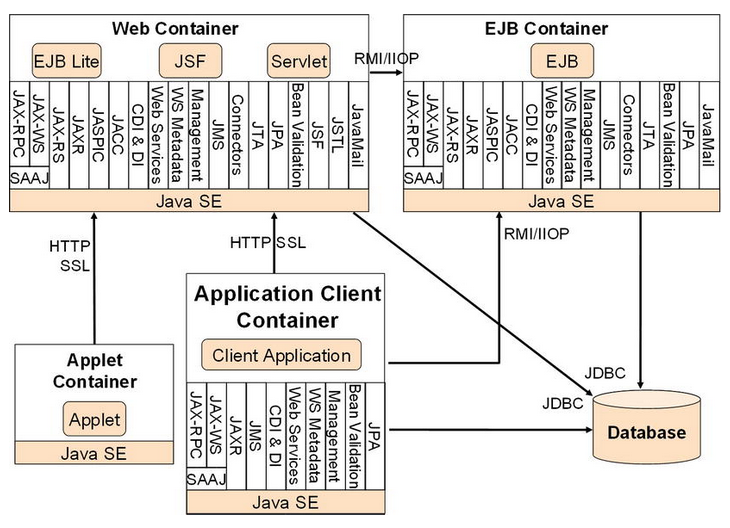
\includegraphics[width=14cm]{kontener-szolgaltatasok.png}
\end{figure}

\section{Annotációk és deployment descriptorok}

Ahogy az előbb írtam, a konténerek szolgáltatásokat nyújtanak a komponensek számára. Ezek a szolgáltatások alapbeállításokkal rendelkeznek. Például egy entitás osztály egy String típusú tagváltozója varchar2(255) típusú mezőbe fog leképződni az adatbázisban. Abban az esetben, hogyha ezt meg kívánjuk változtatni, meta-adatként kell megadnunk a forráskódban, vagy egy külső fájlban. Forráskódban egy annotációt használva jelezzük az alapbeállításon való változtatást, amikor pedig egy külső fájlban tesszük ezt meg egy deployment descriptor-t alkalmazunk. Ez a deployment descriptor egy XML fájl, amiben a meta-adatok leírása található. A Java EE 6 óta, amikor is beletettek az annotációkat a platform eszközei közé, az általános trend az annotációk használata, mivel ez jóval kevesebb írást igényel, illetve a meta-adat azon a helyen kerül rögzítésre, ahol kifejti a hatását, így egyszerű kezelhetőséget nyújt. Hátránya, hogy egy annotációban megadott érték megváltoztatása a kód újra fordítását igényli. Deployment descriptor esetében elegendő az xml fájlban átírni az értéket.
A két meta-adat megadási mód közül a deployment descriptor rendelkezik magasabb precedenciával. Tehát ha egy meta-adat értéket annotációval is megadtunk, illetve deployment descriptort is alkalmazunk, de abban más értéket állítottunk be, akkor az felülírja az annotációban megadott értéket, és az fogja kifejteni a hatását.

\chapter{Az alkalmazás}

\section{Az adatbázismodell}

Az adatbázismodell 15 darab táblából áll. Ezek közül 12 forgalmi tábla. Forgalmi tábláknak azokat a táblákat nevezzük, amelyek egy entitásra jellemző adatokat tartalmaznak. Például, az általam használt táblák közül az APPLICATIONUSER tábla egy forgalmi tábla, mert egy felhasználó adatait(neve, felhasználóneve, jelszava, stb) tartalmazza. Egy jól megtervezett adatbázismodellben a modell összes táblája közvetlenül kapcsolódik legalább egy másik táblához, és közvetve az összeshez. Ez azt jelenti, hogyha gráfként ábrázoljuk a modellt, amiben a táblák a csúcsok, és két csúcs akkor van összekötve a gráfban, ha az általuk reprezentált táblák között bármilyen(egy-egy, egy-több, több-több) kapcsolat van, és a gráf bármely pontjából vezet út bármely másik pontjába. A forgalmi táblák mellett kapcsolótáblákról is beszélünk. Ezek azok a táblák, amelyek két több-több kapcsolatban álló tábla közé ékelődnek be, méghozzá azért, hogy eltárolják, hogy az egyik tábla mely entitása mely másik táblabeli entitásokhoz kapcsolódik, és fordítva. Az alkalmazásomban által használt adatbázisban egy kapcsolótábla a JND\_ORDERS\_SERVICES. Ez a tábla az ORDERS és a SERVICES tábla között teremt kapcsolatot, melyhez a két oszlopát használja fel. Az ezekben szereplő értékek a idegen kulcsok, melyek elsődleges kulcsok a kapcsolat két oldalán álló táblákban. Egy sorbeli két mezőérték mutatja meg, hogy az egyik tábla mely rekordja a másik tábla mely rekordjához kapcsolódik. Például, ha az ORDER\_ID\_FK mező értéke 9, és a SERVICE\_ID\_FK-é 12, egy másik rekordban pedig 9 és 14, egy harmadikban pedig 10 és 14 ez a két érték, akkor az azt jelenti, hogy a 9-es ID-jű Order rekord a 12 ID-jű, és a 14-es ID-jű Service rekordhoz is kapcsolódik, a 14-s ID-jű Service rekord pedig a 9-es és 10-es ID-jű Orderhez.


A modell ER diagrammja a következő képen látható:

\begin{figure}[!h]
	\centering
	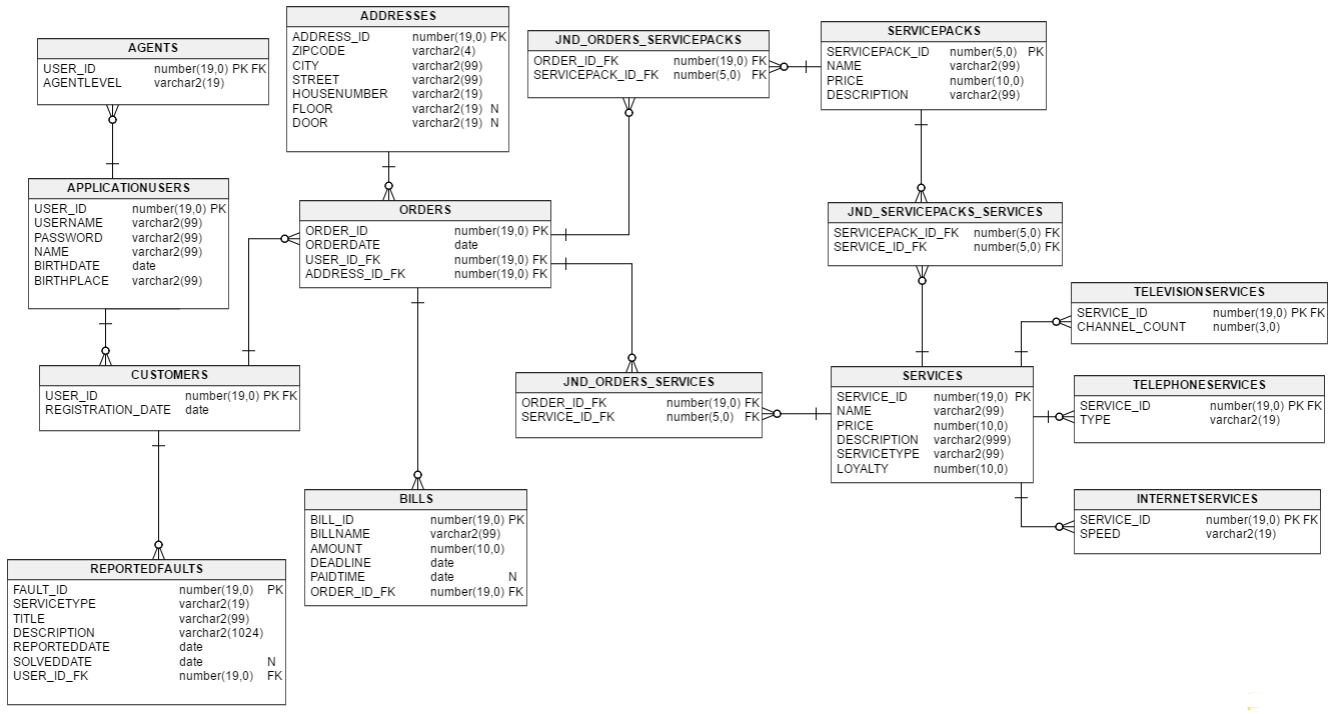
\includegraphics[width=14cm]{adatbazis-modell.png}
\end{figure}


Az adatbázis felhasználókról, bejelentett hibákról, rendelésekről és a rendelésekhez kapcsolódó adategyüttesekről tárol értékeket. Ez utóbbiak a megrendelt szolgáltatások és/vagy szolgáltatáscsomagok, a rendeléshez tartozó cím amelyre a megrendelt szolgáltatásokat bekötik, és a számlák, amelyek a megrendelés véglegesítése után rögtön le is generálódnak.

A felhasználói adatok az APPLICATIONUSER, az AGENTS és a CUSTOMERS táblában szerepelnek. Az APPLICATIONUSER tábla egy "őstábla", amely mindazokat a mezőket tartalmazza, amik az Agent típusú és a Customer típusú felhasználók leírására szolgálnak. Az Agent-ök egyedi jellemzőit az AGENTS tábla mezői jelentik. A Customer-ök egyedi adatai pedig a CUSTOMERS táblába kerülnek bele. Hogy mi miatt van ez, és hogy miért jó ez, arról egy másik részben fogok írni.

A megrendelések jellemzőit az ORDERS táblában találjuk. A megrendeléshez cím (város, utca, stb) tartozik, amelyek egy a számukra fenntartott táblában -- amely az ADDRESSES -- kapnak helyet. Ennek oka, hogy amennyiben egy címre több megrendelés is érkezne, elég a címet összeállító adatokat egyszer eltárolni, így elkerüljük az adatok fölöslegesen sokszori eltárolását, és ezáltal gazdaságosabban használjuk fel a tárhelyünket. Egy megrendeléshez nem a cím részleteit(utca, házszám, stb), hanem a cím rekord elsődleges kulcsát tároljuk el idegen kulcsként, amivel hivatkozhatunk rá.

A szolgáltató az általa nyújtott szolgáltatásokból szolgáltatáscsomagokat rak össze. Egy szolgáltatása akár több csomagban is szerepelhet. Nyilvánvalóan egy szolgáltatáscsomag több szolgáltatásból áll. A szolgáltatások közös adatait a SERVICES tábla, a szolgáltatáscsomagok adatait a SERVICEPACKS tábla tárolja. A szolgáltatáscsomagok és a bennük lévő szolgáltatások összerendelését a JND\_SERVICEPACKS\_SERVICES kapcsolótábla tárolja. A különböző típusú (Internet, KábelTV, Telefon) szolgáltatások típusjellemző adatait az INTERNETSERVICES, a TELEVISIONSERVICES és a TELEPHONESERVICES táblákban találjuk. Az elv ugyanaz, mint a felhasználói adatok tárolására használt táblák kialakításánál.

A szolgáltatásokat és szolgáltatáscsomagokat kapcsolótáblák kötik a megrendelésekhez. Ezek a táblák az idegen kulcsokon kívül mást nem tartalmaznak, neveik: JND\_ORDERS\_SERVICES és JND\_ORDERS\_SERVICEPACKS.

A modell utolsó táblája a BILLS nevű tábla. Ezen táblabeli rekordok tartalmazzák a megrendelések után létrejövő számlák adatait. Számlanév, az összeg, amiről a számla szól, a befizetési határidő, amely minden esetben a következő hónap 5-e, és a befizetés ideje. Ezen utolsó mezőt, ami egy Date típusú PAIDTIME nevű mező használom fel arra, hogy egy számláról megállapíttassam, hogy be van-e már fizetve. Amennyiben ezen mező értéke null, úgy tudjuk, hogy még befizetetlen számláról van szó, ha pedig egy dátum érték szerepel benne, egyértelmű, hogy befizetett. Az előbb leírtak alapján a NOTNULL megszorítást erre a mezőre nem raktam rá. A rekord ORDER\_ID\_FK idegen kulcsa elárulja, hogy melyik megrendelésről szól a számla.

\section{A projekt összeállítása}

A projekt vázának egy Vaadin archetípust\footnote{\url{https://vaadin.com/maven\#dependencies}}, nevezetesen a vaadin-archetype-application archetípust használom. Ez az archetípus egy kiindulási alapot szolgáltat, amelyhez az EJB-k, entitások és egyéb Java objektumok, illetve a konfigurációs fájlok, mint például a persistence.xml, hozzáadása az alkalmazás elkészüléséhez vezet.
Ahhoz, hogy ezen archetype alapján egyszerűen létrehozzam a projektet, egy új projektet hozok létre, amely egy maven-es projekt, és a projekt létrehozása során megadom, hogy archetype alapján jöjjön létre a projekt. Ehhez meg kell adni az archetype jellemzőit: groupID, artifactId, és a verzió. \href{https://vaadin.com/maven#dependencies}{Mindezek a Vaadin honlapján elérhetőek.} Jelen esetben ezek a következőek: groupId: com.vaadin, artifactId:vaadin-archetype-application version: 7.6.2 . Az archetype kiválasztása után a saját alkalmazásunk groupId-ját és artifactID-ját kell megadnunk. Én groupdId-nak a com.szakdolgozat, artifactId-nak pedig a szer-t választottam. Ezen adatok megadása után az IDE letölti a maven központi repository-jából a archetype-ot, mint függőséget, és ez alapján legenerálja a projektet. Ezután rendelkezésünkre áll egy kiindulási projekttartalom, ami mindössze egy UI java objektumot, egy gwt.xml-t és néhány a kinézetre(forntend) vonatkozó .scss-t tartalmaz, egy struktúrált mappaszerkezetben.

Ezután az alkalmazás IDE-ből deployolhatóságát állíttam be. Ehhez egy plugin-t használok, amely alkalmazásszerver specifikus. Ez a plugin mavennel könnyen hozzáadható az alkalmazásunkhoz. A 	
\lstinputlisting[caption=WildFly plugin,label=kod-wildfly-plugin]{wildfly-plugin.pas}
sorok pom.xml-hez hozzáadásával a plugin letöltésre kerül, és a projekt részévé válik. Ezután a Maven toolboxban megjelenik a pluginok között, és a wildfly:deploy opció indításával máris deployolásra kerül az alkalmazásszerverünkre. A port és name konfigurációs attribútumok beállításával finomhangolhatjuk a deployolás tulajdonságait. Jelen esetben a 10000-es porton futó administration consol-ú szerverre fog történni a deploy - melynél jelen esetben maga a szerver a 8090-es porton fut - és szer.war néven fog az alkalmazás deployálásra kerülni. Ez utóbbi azt vonja magával, hogy az alkalmazást a localhost:8090/szer URL-en fogjuk elérni. 

Ezt követően az első lépés az adatbázis elérést lehetővé tévő persistence.xml fájl hozzáadása a projekthez, amelyet az src mappa alatt néhány mélységben található resources almappában létrehozandó META-INF mappában kell elhelyezni. Ez az xml file tartalmazza az adatbázis eléréséhez szükséges információkat. Jelen esetben a DataSource nevét, amely az adatbáziskapcsolat kialakításához szükséges információkat tárolja: az adatbázis címe, a bejelentkezéshez szükséges felhasználónév és jelszó.
Emellett ami számunkra fontos ebben az xml-ben, az a table generation strategy. Egy jól megválasztott stratégiával gondoskodhatunk az adatok biztonságáról. Én az update értéket választottam. Ez a stratégia az alkalmazás indulásakor megvizsgálja az adatbázis séma tartalmát, és amennyiben nem talál benne a projektben definiált entitás számára táblát, létrehozza azt. Abban az esetben pedig, amikor egy entitásosztály tagváltozóinak típusa és/vagy a tagváltozókhoz beállított adatbázisbeli jellemzők az adatbázisbeli táblafelépítéssel nincsenek szinkronban, úgy a tábla módosításra kerül, hogy annak jellemzői az entitásosztályban beállított jellemzőket tükrözzék.
Például, ha egy Java osztály, ami egy entitást ír le rendelkezik egy int típusú és mennyiség nevű tagváltozóval, aminek az entitáshoz tartozó táblában nincs megfelelő mező, úgy a tábla egy "ALTER TABLE ..." DDL utasítás automatikus lefutásával módosul, és bővül egy mennyiség nevű mezővel. 

Az ORM műveleteket a Hibernate, egy JPA implementáció fogja végezni. Ennek magja az entitmy manager. Ahhoz hogy ezt a persistence provider-t használni lehessen, függőségként hozzá kel adnunk a projektünkhoz. Ezt a pom.xml szerkesztésével tehetjük meg:

\lstinputlisting[caption=Hibernate függőségek, label=kod-hibernate-dependencies]{hibernate-dependencies.pas}


A fenti kód alapján a maven a központi repositoryból letölti a szükséges JAR-okat, és hozzáadja a projektünkhöz. Így már fogjuk tudni használni a Hibernate-t, amivel az objektumorientált programunk entitásainak világa és a "rekord orientált" adatbázisunk rekordjainak világa közötti átjárást tesszük lehetővé.

\section{Az adatbázis-modell megvalósítása Java Entity-k felhasználásával}

Egy alkalmazás számos dologból épül fel: üzleti logika, felhasználói felületek, más alkalmazásokkal történő kommunikáció, ... , és ezek mellet egy lényeges elem az adat. A pályafutásunk első elkészült szoftvereiben, amik funkciója általában a felhasználó nevének és kedvenc állatának bekérésében kimerült, a kis adatmennyiség miatt, illetve az adat felhasználásának rövid időtartama miatt elegendő volt, hogy ezek csak a memóriában kapjanak helyet. Azonban a gyakorlatban használt alkalmazásuk szinte mindegyike olyan alkalmazás, amely hatalmas mennyiségű adat elérését igényli, amelyek rendszerint egy adatbázisban találhatóak meg. Ezen adatbázisok legtöbbje relációs adatbázis, amely táblákba és azon belül rekordokba rendezve tárolja az adatokat. Mi, amikor egy Java EE alkalmazást készítünk, nem rekordokkal, hanem az objektumorientált világ objektumaival dolgozunk. Emiatt szükségünk van valamire, amik Java oldalon "kézzel foghatóvá", egységbe zárttá teszik az adatokat. Ezek a valamik az entitás osztályok. Ezek olyan osztályok, amelyek egy-egy tagváltozója az adatbázisbeli rekord egy-egy mezőjét reprezentálja. Egy alap entitás osztály implementálása egy java osztály megírását jelenti(Plain Old Java Object - Pojo), amit ellátunk az @Entity annotációval. Ezen annotáció alapján a Java EE-s környezetünk tudni fogja, hogy egy ebből az osztályból létrehozott memóriabeli objektumok az adatbázishoz kapcsolódnak: leképezhetőek abba, törölhetőek onnan, lekérdezhetőek. A leképzést a JPA végzi, ami egy saját lekérdező nyelvet, a  JPQL-t adja az adatbázison futtatható lekérdezések Java oldali elkészítéséhez.

\lstinputlisting[caption=Service entitás osztály,label=Service entitás osztály]{service-entity.java}

A következőkben az általam készített alkalmazás egy entitás osztályán keresztül fogom bemutatni, hogy miként állíthatunk össze és paraméterezhetünk fel egy entitást, amennyiben nem a JPA által adott default értékeket kívánjuk használni, például egy String típusú tagváltozó mappelésekor.


A kód első sora, a már említett @Entity annotáció, amivel azt jelezzük, hogy a POJO-nkat egy entitás osztállyá alakítjuk. Ez egy kötelező annotáció. A második sorban a @Table annotáció került elhelyezésre. Ez az annotáció az entitást fogadó táblához nyújt beállítási lehetőségeket. Itt adhatjuk meg a tábla nevét, amennyiben az az entitás osztály nevétől eltérő. Szintén itt fogalmazhatunk meg megszorításokat a táblához. Mindezek megadása opcionális. Ha a name attribútumnak nem adunk értéket, akkor a létrejövő tábla neve az entitás nevével fog egyezni. A 3. sorban az @Inheritance annotáció látható. Ezt az annotációt azokban az esetekben használjuk, amikor szülő és leszármazott kapcsolatban álló entitásosztályokat akarunk az adatbázisban használni. Jelen esetben ez a Service nevű osztály az ősosztály, amiből 3 leszármazott osztály ágazik le (InternetService, TelephoneService, TelevisionService). Ez az annotáció ugyanebben a formában mindhárom osztály forráskódjában szerepeltetésre kell kerüljön. Az annotáció strategy attribátumával adható meg, hogy melyik öröklődési típust alkalmazzuk. Három stratégia közül választhatunk fejlesztőként, ezek  következőek:
\begin{itemize}
	\item Single-Table-per-Class: Ezt a stratégiát alkalmazva az osztályhiercarchiában lévő összes osztályból készült objektumok egyetlen táblába kerülnek bele. Emiatt ez a tábla tartalmazza az összes oszlopot, ami az osztályok tagváltozóinak tárolására szolgál. 
	\item Joined: Amikor ezt a stratégiát választjuk, az osztályhierarchia összes osztálya számára egy külön tábla jön létre. Az ős osztályok számára készült táblák tartalmazzák az összes olyan mezőt, amik a közös tagváltozók értékeinek tárolására szolgálnak. A leszármazott osztályok táblái így elég, ha csak kifejezetten a leszármazott osztályok által tartalmazott tagváltozók mezőből állnak össze.
	\item Table-per-Concrete-Class: Ezt a stratégiát alkalmazva az osztályhierarchia összes osztálya számára létrejön egy külön tábla, méghozzá úgy, hogy azok az osztály összes tagváltozóját tároló mezőt tartalmazzák.
\end{itemize}

Az alkalmazás által használt adatbázis sémája jelene esetben a Joined stratégia használatát tette szükségessé. Ennek két oka van.
Az egyik ok az, hogy a Service osztály leszármazott entitásinak vannak olyan mezői, amelyek az adatbázisban a not-null megszorítást viselik. Emiatt a Single-Table-per-Class strategy nem működhet, mivel ez lehetetlenné tenné olyan leszármazott osztályból készült rekordok beírását az egyetlen táblába, amelyek nem rendelkeznek olyan mezővel, amire a not null megszorítás érvényben van, mivel nem felelhetnek meg ennek a megszorításnak.
A másik ok, ami miatt a Joined stratégiát alkalmaztam, hogy az adatbázis-modell felépítése és kis mérete miatt nem érdemes bevállalni a modell denormalizását, amivel a Table-per-Concrete-Class stratégia járna.

Az entitásosztály negyedik sorában lévő @DiscriminatorColumn annotáció az ősosztály táblájában lévő egy speciális oszlopának jellemzőit állítja be. Ez a speciális oszlop értéke tárolja minden egyes rekord esetén, hogy az melyik leszármazott osztálybeli rekordhoz tartozik. Ezáltal az entitás objektum elkészítése a megfelelő osztály konstruktorával fog történni, elkerülve a hibás működést.
Ez az annotáció szintén opcionális.

Mindezen meta-adatok megadását követően az entitás osztály tagváltozóinak, konstruktorainak,  gettereinek és settereinek implementálása következik. Ennek módja ugyanaz, mintha egy nem entitás osztályt állítanánk össze. A tagváltozókból leképzett adatbázisbeli mezők jellemzőit a szintén annotációkkal adhatjuk meg. Ezek közül egyetlen egy a kötelező, mégpedig az @Id. Ez az annotáció szolgál jelzésül a fordítónak arra vonatkozólag, hogy melyik tagváltozó lesz a rekord elsődleges kulcsa. Ez egy egyedi azonosító az objektumok azonosításához. Ebben a példában a serviceId nevá tagvoltozó kapta meg ezt az annotációt, így ez lesz az entitás azonosítója. Rögtön az @Id annotáció alatt a @GeneratedValue következik. Ezzel azt a beállítást adjuk meg, hogy mi nem a JPA-ra bízzuk az elsődleges kulcsok generálását a perzisztálás során, így elkerüljük azt a hibalehetőséget, hogy esetleg olyan elsődleges kulcsú objektumot próbáljunk elhelyezni az adatbázis egy táblájában, amivel egy másik már szerepel. A serviceId harmadik annotációja a @Column, amivel az oszlop jellemzőit állíthatjuk a default beállítástól eltérőre. A name attribútummal a mező nevét adhatjuk meg, ami default esetben az entitás tagváltozójának neve. A description nevű tagváltozón további attribútumok megadásával a mezőnév megváltoztatásán túl más alapértékeket is felülírtunk: a nullable = false értékkel azt a megkötést tettük a mezőre, hogy nem vehet fel null értéket, a length = 255-el a Varchar2 típusú mező hosszát a 255-re állítottuk. 

A Service tábla egy olyan tábla, amelyik több-több kapcsolatban áll két másik táblával. Ezt implementálni a következőképpen lehet: Az entitásosztályban létre kell hozunk olyan Collection típusú tagváltozókat, amelyek azon entitásosztály típusú elemeket tárolnak, amelyek a több-több kapcsolat másik oldalán állnak. Például, az adatbázis-modellben szerepel egy Services-Orders táblák közötti több több kapcsolat. Amiatt a Service entitásosztály egy Order-eket tároló Collectiont (jelen esetben List-et) kell hogy tartalmazzon, amit a @ManyToMany annotációval láttam el, az összerendelés típusának megadására. Az annotáció mappedBy attribútumértéke az az Order entitásbeli tagváltozó neve, amelyik az Order oldalon a több-több kapcsolat jelzésére szolgál.

\lstinputlisting[caption=Order entitás kódrészlet,label=Order entitás kódrészlet]{order-entity-part.java}

Mint a beillesztett kódrészletben látható, ez a services tagváltozó. ahhoz, hogy a több-több kapcsolat kiépíthető legyen, ugyanitt, a services tagváltozón definiálni szükséges a rekordok közötti kapcsolatokat eltároló kapcsolótábla adatait. Ezt a @JoinTable annotáció felhelyezésével tettem meg, aminek attribútumként megadtam a kapcsolótábla nevét (name = "JND\_ORDERS\_SERVICES"), és a kapcsolótábla két oszlopának a nevét, amelyek közül az egyik a Service rekord elsődleges kulcsát, a másik pedig az Order rekord elsődleges kulcsát tárolja. Ezzel elkészült a Service és Order táblák közötti több-több kapcsolat kialakítása.

Abban az esetben, ha egy egy-több kapcsolatot szükséges kiépítenünk, hasonló elvet kell hogy kövessünk. A kapcsolat egy oldalán lévő entitásosztályban egy Collection-t kell elhelyeznünk, ami a több oldalon lévő entitás típusának megfelelő elemeket tartalmaz. Ezt a tagváltozót a @OneToMany annotációval kell hogy ellássuk, aminek a mappedBy attribútumát a több oldalon lévő entitásosztályba szereplő, az egy oldalon lévő entitástípusú tagváltozó nevére kell beállítanunk. 
A több oldali entitás egy oldalra mutató tagváltozójára a @ManyToOne annotációt kell hogy felhelyezzük. Emellett a @JoinColumn annotáció használata is kötelező, mivel ezzel az annotációval adunk nevet több oldali táblának annak a mezejének, ami az egy oldali entitás elsődleges kulcsát fogja tartalmazni idegen kulcsként. Az annotáció második attribútuma (referencedColumnName) az idegen kulcsként használt elsődleges kulcs gazdatáblájában használt nevét kell hogy tartalmazza.

Ezennel az adatbázistáblák összeállításához használandó meta-adatok megadásra kerültek.

Fontos még megjegyezni, hogy az entitásosztályoknak mindenképpen rendelkezniük kell default konstruktorral, mivel a JPA az entitásobjektumokat ezzel a konstruktorral példányosítja. Szóval abban az esetben, hogyha definiálunk egy az alap konstruktortól eltérő konstruktort, ami fölülírná a default-at, úgy kézzel ismét meg kell írnunk a paraméter nélküli konstruktort, megelőzve ezzel az alkalmazást működésképtelenségét. 

\section{Az üzleti logika}

Az alkalmazás üzleti logikájául szolgáló programkódot EJB-k formájában írtam meg.
Ezek az EJB konténer-menedzselt Java objektumok. Ez azt jelenti, hogy példányosításukért, inicializálásukért, stb a konténer felel. Ez azt jelenti, hogy a programozónak elég egy @Inject annotációval "befecskendezni" az EJB egy olyan helyen,a hol használni akarja, anélkül, hogy a new kulcsszóval példányosítani azt. Emellett a konténer annyi Bean-t példányosít, amennyi az optimális működéshez szükséges. Amennyiben a web alkalmazás felé rengeteg kérés érkezik a sok kliens miatt, több EJB objektum van jelen a konténerben, kevesebb kérés esetén kevesebb.
Az EJB-knek 3 fajtájuk van:
\begin{itemize}
	\item Stateless: A beanek ezen típusa nem tárol állapotokat, bármelyik klienst bármelyik bean példányt kiszolgálhatja. Olyan task-ok kezelésére hívatottak, amik csakis a bemenő paraméterekkel dolgoznak, és azok alapján a működésük az elvárt eredményt fogja magával hozni.
	\item Stateful: Ezek a beanek képesek állapotokat tárolni, amelyek ugyanazon kliens számos metódushívása során is felhasználható. Ez akkor hasznos, amikor egy task elvégzését több lépésben kell elvégezni.
	\item Singleton: A singleton beanek olyan beanek, amelyek közös használatra vannak megosztva a konténer által kiszolgált kliensek között, és az alkalmazásban csakis egy példány van jelen belőlük.
\end{itemize}

Egy POJO-t a @Stateless, a @Stateful vagy a @Singleton annotációk egyikével alakíthatunk EJB-vé. Természetesen ezek közül egy időben csak egyet használhatunk ugyanazon EJB esetén. Az alábbi példakódban egy egyszerű Singleton Bean implementációja látható:

\lstinputlisting[caption=DateFormatConverter EJB,label=DateFormatConverter EJB]{dateformatconverter-class.java}

Ezt a beant közös használatra terveztem az alkalmazás részeinek számára, emiatt Singleton típusú beannek állítottam be. A bean 3 metódust tartalmaz, amelyek egy paraméterül kapott dátumot más és más formátumú dátumsztringgé konvertálnak át. Látható, hogy ez egy a Java SE-ben megszokott osztálydefiníciótól mindössze annyiban tér el, hogy a egy annotáció felkerült rá. 

A használat helyén elegendő az @Inject annotációval befecskendezni egy példányt a beanből, amihez a típust és a változónevet szükséges még megadnunk:

\lstinputlisting[caption=Injectálás ,label=Injectálás]{inject.java}

Ezután a Java SE-ben megszokott módon elérjük az objektum metódusait:

\lstinputlisting[caption=Injectált bean metódusának meghívása,label=Injectált bean metódusának meghívása]{injectalt-ejb-hasznalat.java}

\section{Adatbázisműveletek a JPA igénybevételével}

Mint már említettem, egyes konténerek különféle szolgáltatásokat nyújtanak a bennük futó komponensek számára. Ezek közül az egyik leggyakrabban használt szolgáltatás a JPA.
A JPA az objektumorientált világ és a relációs világ között teremt kapcsolatot. Középpontjában az entity manager van, ami az entitások állapotát és életciklusát kezeli, és lekérdezéseket tesz lehetővé. Ez felelős az entitás példányok létrehozásáért és eltávolításáért, valamint ez találja meg az entitásokat az adatbázisban az elsődleges kulcsuk alapján. Lockolhat entitásokat a konkurens hozzáférés megvalósításáért, illetve rendelkezik egy JPQL nevű lekérdező nyelvvel, amivel SQL  utasításokat hajthatunk végre a JPQL szintaktikával megírt parancsokkal. A gyakorlatban ez úgy valósul meg, hogy egy persistence provider implementálja az EntityManager interfacet, aminek a metódusai SQL utasításokat generálnak és futtatnak le. Számos persistence provider érhető el open-source formában: Hibernate, OpenJPA, EclipseLink.

A következő példakóddal néhány az entity manager által kínált műveletet mutatok be, amiben az is láthatóvá válik, hogy a JPQL szintaktikája mennyire közel áll a natív SQL szintaktikájához.

\lstinputlisting[caption=JPA-EntityManager,label=JPA-EntityManager]{entitymanager.java}

Ahhoz, hogy egy entity managert használni tudjunk egy beanben, először elérhetővé kell tennünk egy példányát az EJB-ben. Ezt a @PersistenceContext annotációval ellátott EntityManager deklarációval tehetjük meg. Ekkor a @PersistenceContext unitName attribútumában megadott persistence unitban megjelölt adatbázis sémához hozzáférő entity managert kapunk. A bean doRegistration metódusa egy egyszerű metódus, ami paraméterül megkap egy ApplicationUser típusú objektumok. A metódus lefutása ezt az objektumot helyezi el az adatbázisban azáltal, hogy meghívja az entity manager persist() metódusát a user paraméterrel. Ennek hatására amennyiben az entitás még nem szerepel az adatbázisban, úgy az perzisztálásra kerül, ellenkező esetben egy EntityExistException kivételt kapunk.

A bean második metódusában egy JPQL query futtatására kerül sor. Ehhez elsőkörben egy TypedQuery típusú objektumot kell létrehoznunk, amit az entity manager createQuery metódusa ad visszatérési értékül. Ezen metódus paraméterlistájában kell megadnunk a lekérdezést JPQL nyelven megfogalmazva. Lekérdezésről lévén a SELECT utasítást kell ehhez használjuk. A FROM kulcsszó után nem a tábla nevét, hanem az entitásosztály nevét kell megadnunk, azét az entitásosztályét, amilyen típusú entitás-on hajtjuk végre a lekérdezést. Ezután egy "jelölőt" kell megadnunk, amivel a lekérdezésben erre a típusra tudunk hivatkozni. Az entitás(ok) összes mezejének lekérdezéséhez ezt a jelölőt kell használnuk az SQL-ben megszokott * helyett. A lekérdezéshez feltételeket fogalmazhatunk meg, amiket a WHERE kulcsszóval kapcsolunk a SELECT után. Több feltétel is használható, amelyeket az AND és OR logikai operátorokkal köthetünk össze. Dinamukissá tehetjük a lekérdezéseket azáltal, hogy a feltételekbe nem beégetett értékeket adunk meg, hanem azokba paraméterül kapott értékeket helyettesítünk be. Ehhez a feltétel jobb oldalára egy ":"-val kezdődő paraméternevet kell megadnunk, amelybe egy konkrét értéket a query setParaméter metódusával állíthatunk be.

Az elkészült query-t attól függően, hogy milyen eredményhalmazt várunk, különböző metódusokkal futtathatunk le. Jelent Esetben a getSingleResult() metódus meghívásával fut le a query, amitől azt várom, hogy egyetlen objektumot fog visszaadni. Amennyiben nincs a feltételeket kielégítő rekord az adatbázisban, úgy kivételt fog dobni az entity manager.
A lekérdezést emellett a getResultList() metódussal is futtathatjuk, amennyiben azt várjuk, hogy több objektumot eredményezni fog a lekérdezés, illetve a getFirstResult() metódust is alkalmazhatjuk, ami 1-nél nagyobb eredményhalmaz esetén a legelső objektumot fogja számunkra szolgáltatni.

Amennyiben update vagy delete DML utasítást akarunk futtatni, úgy az exectueUpdate() metódussal futtathatjuk a query-nket, ami a módosított/törölt rekordok számát adja visszatérési értékül. 

\section{A megjelenítésre kerülő felületek}

A felhasználók által látot képernyőket Vaadin-nal készítettem el. A Vaadin egy felhasználói felületek elkészítésére való keretrendszer, ami rengeteg Java szerver oldali előre definiált komponenst tartalmaz, amiket a programozók a képernyők összeállítására használhatnak. 

Minden egyes képernyő egy View nevű java osztály, amelyben a képernyőn használt komponenseket gyújthetjük össze, azért, hogy azokat a képernyőn helyezzük el. Ezek a komponensek különfelé Layout-ok, gombok, panelek, beviteli mezők, táblázatok, és így tovább. Például egy a képernyőre kihelyezendő formot egy form komponens példányosításával hozhatunk létre, amihez a formba kihelyezendő beviteli mezőket és gombokat elhelyezve a form teljes tartalmát egyetlen objektumként kezelhetjük.

\subsection{UI}

A UI a komponens hierarchia legtetején álló komponens. Minden egyes böngésző ablakbeli 
Vaadin példánynak egy saját IU-a van. Egy UI megjeleníthet egy egész böngésző ablaknyi tartalmat, vagy lehet egy html oldal része, amibe egy Vaadin alkalmazást ágyaztak be.
Egy új UI példány tipikusan akkor készül el, amikor egy felhasználó megnyitott egy URL egy böngésző ablakban, ami például egy VaadinServlet-re mutat.
Miután a UI elkészült, az inicializálására kerül sor, ami az init(VaadinRequest) metódus használatával megy végbe. Ez a metódus a fejlesztők által felülírható, hogy komponenseket adjanak hozzá a user interface-hez, és hogy nem-komponens funkciókt inicializáljanak.
A komponens hierarchiát azáltal kell inicializálnunk, hogy egy komponenst, ami a fő layout-ot tartalmazza, vagy egyéb más tartalmú view-t átadunk a setComponent(Component) metódusnak, vagy pedig a UI konstruktorának.

\subsection{View}

A Vaadin View osztálya képernyők elkészítését teszi lehetővé azáltal, hogy a képernyőt, mint egy objektumot állítunk össze. A View osztály rendelkezik egy enter(ViewChangeEvent) metódussal, amely az oldalra navigálás után kerül meghívásra, ezáltal ez a metódus szolgál arra, hogy a metódus törzsébe írt kódsorokkal, illetve metódushívásokkal előállítsuk az oldal éppen azzal a tartalommal, amit a felhasználónak az adott pillanatba látnia kell.

\subsection{A View-k összeállítása}
A képernyők elkészítéséhez először elkészítettem egy AbstractView osztály, amiben elhelyeztem azokat az elemeket, amik az összes, a felhasználók által látott képernyőn megjelennek. Ezek a következők
\begin{itemize} \hypertarget{leiras-kepernyoteruletek}{}
	\item A logó számára fenntartott terület: Ez a komponens egy képet jelenít meg, amely minden egyes képernyő bal felső sarkában jelenik meg.
	\item "LoginBox": Ez a komponens a bejelentkezés funkcióhoz kapcsolódik, és a jobb felső sarokban kapott helyet. Abban az esetben, hogyha egy nem bejelentkezett felhasználó jár az oldalon, abban az esetben egy két beviteli mezős panel jelenik meg benne, ahol a bejelentkezési adatokat lehet megadni, vagy a regisztrációs oldalra eljutni az itt lévő link által, ha pedig bejelentkezett felhasználóként látjuk a képernyőt, akkor egy egyszerű üdvözlő szöveg jelenik meg itt.
	\item Menüsor: A képernyő bal oldalán, a logó alatti területen a menüsor található. Ez egy olyan komponens, ami minden esetben megjelenik a képernyőn, tartalma viszont attól függően, hogy milyen típusú felhasználó van bejelentkezve változik.
	\item Tartalom: A képernyő jobb alsó részén az éppen kiválasztott menüponthoz kapcsolódó tartalom jelenik meg. Emiatt az abstract ősosztályban csak egy üres, tartalom nélküli layout generálódik ide, aminek a tartalma a leszármazott osztály afterEnter() metódusában tevődik össze.
\end{itemize}


Ahány képernyő van, annyi AbstractView-ból leszármazó osztály implementáltam a képernyők egyedi tartalmának legenerálásához.

Ezen osztályok felhasználásával a képernyők a következő mechanizmus során állnak elő:
\begin{enumerate}
	\item A felhasználó beírja a böngészőbe címsorában az alkalmazás elérését lehetővé tévő URL-t, vagy amennyiben már az oldalak között böngész, rányom egy menüpontra, vagy funkciógombra.
	\item Ezután  meghatározársra kerül, hogy melyik view-t kell megjeleníteni a képernyőn.
	\item Lefut a View-ok absztrakt ősosztályának enter() metódusa, aminek hatására előáll a képernyők default komponenstartalma, azaz az előbb említett \hyperlink{leiras-kepernyoteruletek}{négy képernyőterület.}
	\item Az enter metódus meghívja az afterEnter() metódust, amik a leszármazott osztályokban override-olt metódusok, amik így a konkrét view által megjelenítendő tartalommal töltik fel azokat a komponenseket, amelyek az egyediségük miatt az abstract osztály enter() metódusának futása során nem töltődtek fel tartalommal.
\end{enumerate}

A dinamikus tartalmak összeállításához számos esetben van adatbázishoz fordulás. Ezekben az esetekben a leszármazott view osztályokba injectált bean-ek metódusai azok, amik az adatbázis műveleteket elvégzik, és olyan tartalmat hoznak a leszármazott view-okba, hogy azok már elkészíthetik ezáltal a képernyő teljes tartalmát. Példa erre a szolgáltatások képernyő, amelyet a ServicesView állít elő. Ez esetben szükség van a szolgáltatások listájának táblázatban történő megjelenítésére.
A listázás a szolgáltatás típusának megadása után történik meg. Alapból a telefonszolgáltatások típus van kiválasztva. Az aktuálisan kiválasztott szolgáltatástípus alapján a TableContentHandlerBean egy metódusa fog lefutni, ami összegyűjti az adatbázisból a kiválasztott szolgáltatástípusba tartozó szolgáltatásokat, és a lista alapján előállít egy IndexedContainer példányt, amely példány a szolgáltatások jellemzőit tartalmazza egy rendezett formában, amelyet így a ServicesView-on lévő Table-nek datasourceként beállítva elérhetővé válnak a szolgáltatások jellemzői a táblázatban megjelenve.
Ennek megvalósítását a következő kódrészlet adja:

\lstinputlisting[caption=TableContentHandler EJB,label=TableContentHandler EJB]{tablecontenthandlerbean.java}

A @Stateful annotációval ellátott POJO-nk EJB-ként fog rendelkezésre állni a Web Konténerben. Ezen példányok egyike fogja kiszolgálni a ServicesView objektumbeli metódushívást. A beanbe első körben egy EntityManager került injektálásra, ami az adatbázis műveletek használatához szükséges. Emellett jópár metódus került még megírásra, amelyek többféle helyen használt táblázatok feltöltéséhez állítanak elő IndexedContainer példányok. Ezek közül az egyik a makeTelephoneIndexedConatiner() metódus, amelyik a telefonszolgáltatások táblázat sorait tartalmazza. A táblázat összes oszlopát egy-egy ContainerProperty-ként lehet hozzáadni az IndexedContainerhez. Ehhez három paraméter megadása kötelező, az egyik az oszlop neve, amelyet a felhasználók látni fognak. A második az oszlopba kerülő értékek típusa. Amennyiben egy Item egy mezőértékének az itt megadottól eltérő típusú értéke próbálnánk beállítani, úgy kivétel keletkezik. A harmadik paraméter az oszlopba kerülő alapérték, amennyiben azt explicit módon nem állítanánk be. Ezen paraméterek megadásával előállt egy váz, amelyet adatokkal (sorokkal) tölthetünk fel ezután.
Mivel feltöltéshez használt adatok adatbázisból érkeznek, emiatt egy lekérdezés futtatása szükséges, amelyet a TypedQuery létrehozása és futtatása által teszek meg. Az összes telefonszolgáltatás megjelenítésére szükség van a képernyőn, így a TelephoneServices tábla teljes tartalmának kiolvasása szükséges, azaz az összes rekord összes mezőjét eredményül adó JPQL query megfogalmazását kell megejteni. Ez a következőképpen néz ki: "SELECT s FROM TelephoneService s". A query által adott visszaadott objektumok TelephoneService típusúak lesznek, mivel ezen osztály táblájából olvastuk fel az entitások összes mezőjét. Így ezeket az objektumokat egy TelephoneService elemeket tároló listában lehet például letárolni. Miután a lista rendelkezésre áll, minden egyes eleme alapján egy új Item-et kell hozzáadni az IndexedContainer-hez, méghozzá úgy, hogy minden egyes Property-be a helyes érték kerüljön. Tehát például az "Ár" nevű propertybe egy Integer értéket kell tennünk, méghozzá azt az Integer-t, ami a TelephoneService objektum ár tagváltozójának az értéke. Egy új Item egy új sort fog jelenteni a táblázatban.
A metódus végén nincs más dolgunk, mint visszatérni az összeállított IndexedContainer objektummal.

A hívás a következő kódrészletben látható módon történt, aminek a második sora a services nevű Table komponensnek állítja be tartalomként a metódushívás eredményeképpen létrejött IndexedContainer-t.

\lstinputlisting[caption=Table tartalom beállítása,label=Table tartalom beállítása]{datasource-beallitas.java}


\chapter{Összegzés}

Az alkalmazás és a szakdolgozat elkészítése során úgy vélem sikerült egy erős alapszinten megismerkednem a Java Enterpreise Edition-nel, és mindeközben megismerkedni egy szoftver elkészítésének nehézségeivel, buktatóival. Szembesültem azzal, hogy sokat számít az, hogy előre pontosan megtervezzünk egy-egy funkciót, mert ha például egy már elkészített adatbázis modellen utólag változtatunk, és még ha csak egy táblanév átnevezésről is van szó, az hibához vezethet, amelynek megtalálása nagyságrendekkel több időt vesz igénybe mint a hiba kijavítása.
Összességében örülök, hogy ezzel a témával foglalkozhattam, és hogy sikerült elkészítenem a szoftvert.


\begin{thebibliography}{1}
\bibitem{cimke} \textsc{Antonio Goncalves}: Beginning Java EE 7, Apress, Milton Keynes, 2013.
\end{thebibliography}
\end{document}
